\chapter*{2 Versuchsdurchführung und Auswertung}
\addcontentsline{toc}{chapter}{2 Versuchsdurchführung und Auswertung}
\setcounter{chapter}{2}
\setcounter{section}{0}
\setcounter{subsection}{0}

\section{Versuch 1: Strom-Spannungs Kennlinien}

    \subsection{Versuchsaufbau und -durchführung}

        Versuch 1 behandelt die Strom-Spannungs Kennlinien von Widerständen und Glühbirnen. Dazu wird der Versuchsaufbau aus Abbildung \ref{fig:versuch1} verwendet. Im ersten Teil des Versuch wird die Spannung und die Stromstärke an dem markierten Stellen gemessen und festgehalten. Im zweiten Teil des Versuchs wird die Glühbirne durch einen Ohm'schen Widerstand ersetzt und die Messung wiederholt. Der Widerstand beträgt $R = 1\ \mathrm{k\Omega}$. Diese Messwerte werden ebenfalls festgehalten. In einem $U$ über $I$ Diagramm werden die Messwerte analysiert und die Steigung um den Spannungswert $U = 0\ \mathrm{V}$ bestimmt.
        Im letzten Teil wird für jedes Wertepaar die elektrische Leistung $P$ berechnet und in einem $R$ über $P$ Diagramm aufgetragen.

        \begin{figure}[ht!]
            \centering
            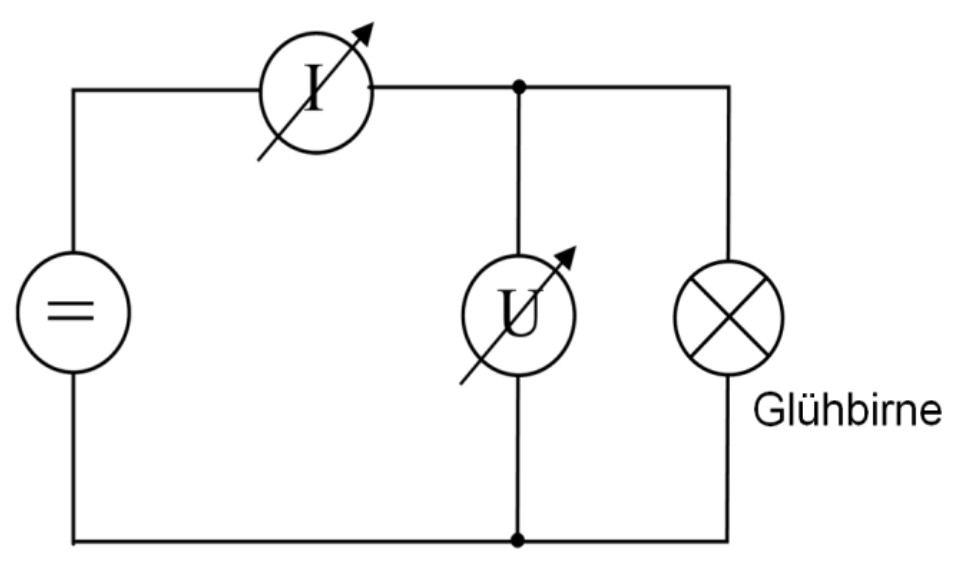
\includegraphics[width=0.5\textwidth]{bilder/Physik_01.png}
            \caption{Versuchsaufbau für Versuch 1}
            \label{fig:versuch1}
        \end{figure}
\newpage
    \subsection{Ergebnisse}

        \begin{table}[ht!]
            \centering
            \begin{tabular}{|l|l|l|l|}
                \hline
                $U$ in $\mathrm{V}$ & $I$ in $\mathrm{mA}$ & $R$ in $\mathrm{\Omega}$ & $P$ in $\mathrm{mW}$\\
                \hline\hline
                $0,00$ & $0,00$ & k.A. & $0,0$\\
                \hline
                $0,50$ & $1,40$ & $357,14$ & $0,7$\\
                \hline
                $1,00$ & $2,60$ & $184,62$ & $2,6$\\
                \hline
                $1,50$ & $3,40$ & $441,18$ & $5,1$\\
                \hline
                $2,00$ & $3,90$ & $512,82$ & $7,8$\\
                \hline
                $4,00$ & $5,70$ & $701,75$ & $22,8$\\
                \hline
                $6,00$ & $7,30$ & $821,92$ & $43,8$\\
                \hline
                $8,00$ & $8,70$ & $919,54$ & $69,6$\\
                \hline
                $10,00$ & $10,00$ & $1000,00$ & $100$\\
                \hline
                $12,00$ & $11,30$ & $1061,95$ & $135,6$\\
                \hline
                $14,00$ & $12,40$ & $1129,03$ & $173,6$\\
                \hline
                $16,00$ & $13,50$ & $1185,19$ & $216$\\
                \hline
                $18,00$ & $14,50$ & $1241,38$ & $261$\\
                \hline
                $20,00$ & $15,50$ & $1290,32$ & $310$\\
                \hline
            \end{tabular}
            \caption{Messwerte für die Glühbirne}
            \label{tab:gluehbirne}
        \end{table}

        \begin{table}[ht!]
            \centering
            \begin{tabular}{|l|l|l|l|}
                \hline
                $U$ in $\mathrm{V}$ & $I$ in $\mathrm{mA}$ & $R$ in $\mathrm{\Omega}$ & $P$ in $\mathrm{mW}$\\
                \hline\hline
                $0,00$ & $0,00$ & k.A. & $0,0$\\
                \hline
                $0,50$ & $0,50$ & $1000,00$ & $0,3$\\
                \hline
                $1,00$ & $1,00$ & $1000,00$ & $1,0$\\
                \hline
                $1,50$ & $1,50$ & $1000,00$ & $2,3$\\
                \hline
                $2,00$ & $2,00$ & $1000,00$ & $4,0$\\
                \hline
                $4,00$ & $4,00$ & $1000,00$ & $16,0$\\
                \hline
                $6,00$ & $5,90$ & $1016,95$ & $35,4$\\
                \hline
                $8,00$ & $7,80$ & $1025,64$ & $62,4$\\
                \hline
                $10,00$ & $9,80$ & $1020,41$ & $98,0$\\
                \hline
                $12,00$ & $11,80$ & $1016,95$ & $141,6$\\
                \hline
                $14,00$ & $13,70$ & $1021,90$ & $191,8$\\
                \hline
                $16,00$ & $15,70$ & $1019,11$ & $251,2$\\
                \hline
                $18,00$ & $17,70$ & $1016,95$ & $318,6$\\
                \hline
                $20,00$ & $19,70$ & $1015,23$ & $394,0$\\
                \hline
            \end{tabular}
            \caption{Messwerte für den Widerstand}
            \label{tab:widerstand}
        \end{table}

        \begin{figure}[ht!]
            \centering
            
            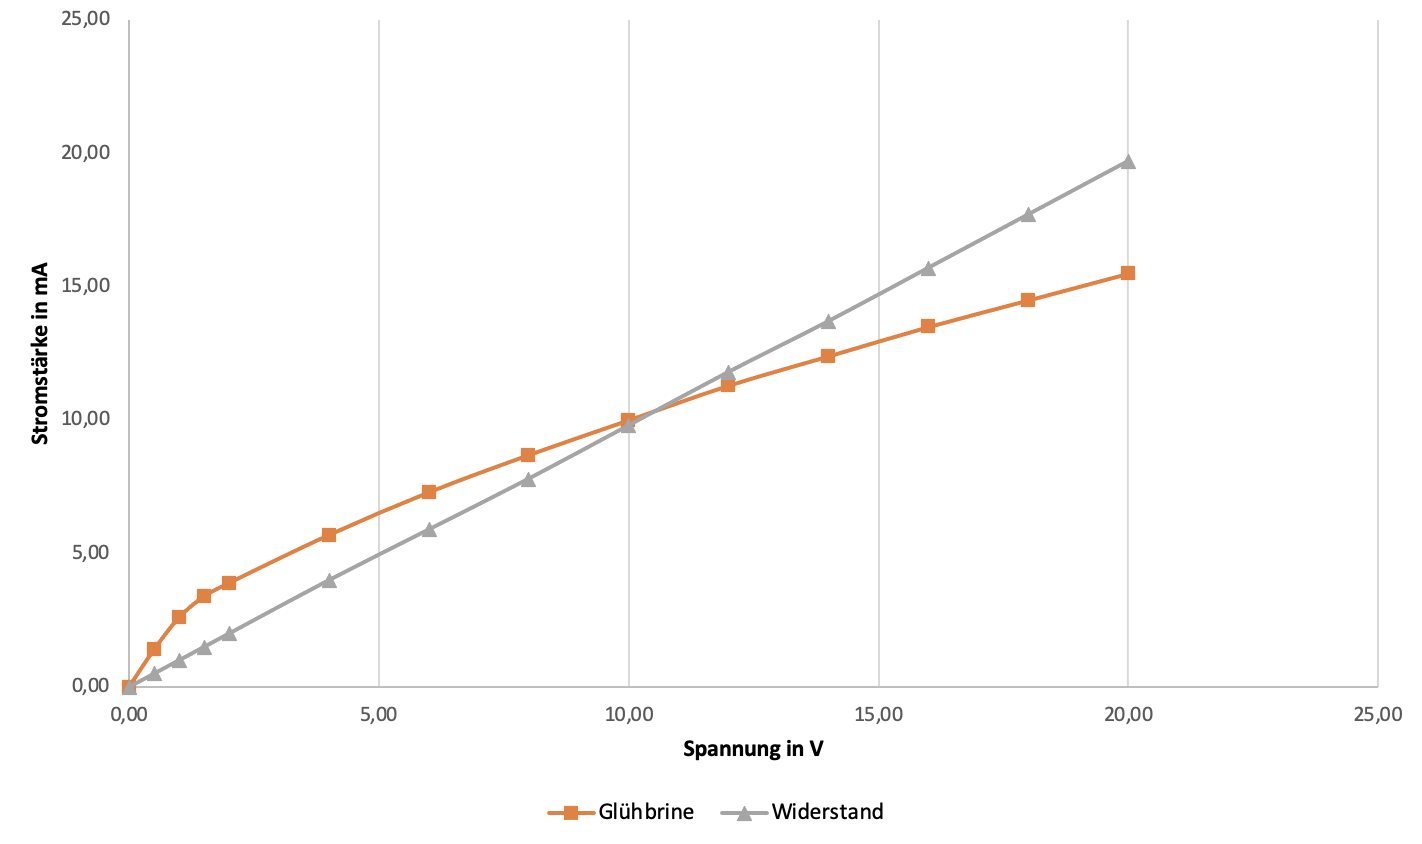
\includegraphics[width=0.5\textwidth]{bilder/Physik_02.png}
            \caption{$U$ über $I$ Diagramm für Glühbirne (orange) und Widerstand (grau)}
            \label{fig:wertev1}
        \end{figure}
\newpage
        \begin{figure}[ht!]
            \centering
            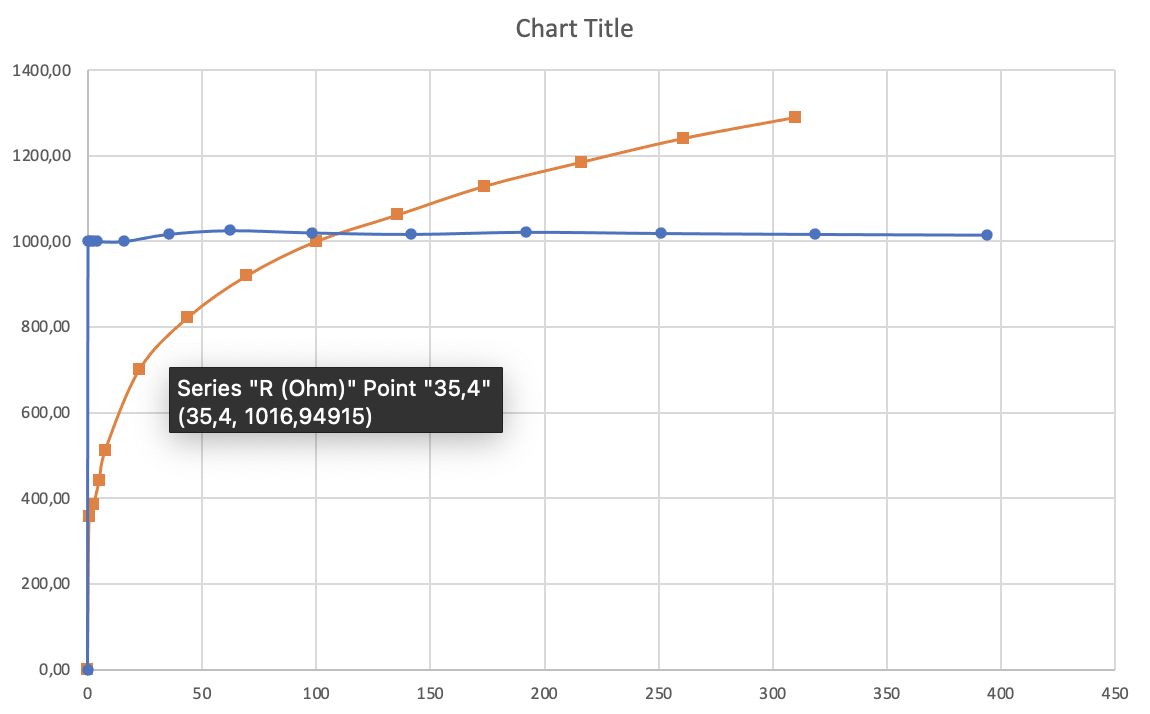
\includegraphics[width=0.5\textwidth]{bilder/Physik_03.png}
            \caption{$R$ über $P$ Diagramm für Glühbirne (orange) und Widerstand (blau)}
            \label{fig:wertev2}
        \end{figure}

      Die Steigung einer Gerade, hier von der Grauen aus dem Schaubild \ref{fig:wertev1}, lässt sich mithilfe der Formel \ref{eq:steigung} berechnen. Dabei entspricht die Steigung R dem Widerstand. $\Delta x$ entspricht der Spannung in Volt und $\Delta y$ der Stromstärke in Ampere. 
      
     \begin{center}
     	\begin{equation}
      	\label{eq:steigung}
      	R = \frac{\Delta y}{\Delta x}
      \end{equation}
     \end{center}
     
     Wählt man nun geschickt $\Delta x= 5V$  $\Delta y=5A$ so erhält man den Widerstand $R = 1 \Omega$

    Man kann aus den Diagrammen so wie den berechneten und gemessenen Werten noch weitere Erkenntnisse ziehen. Zum einen sieht man das im Diagramm \ref{fig:wertev1} die steigende Spannung keinen Einfluss auf den Widerstand hat, während der Widerstand bei der Glühbirne steigt. Dies liegt daran, dass die Glühbirne sich stark erwärmt (Glühdraht) und wenn sich Metalle erwärmen die Atome in Schwingungen geraten was wiederrum zu mehr Kollisionen der Elektronen zur Folge hat. Und da mehr Kollision = höhere Widerstand steigt der Widerstand der Glühbirne (O'hmsches Gesetz). 
    
    Beim Widerstand sollten sich die Werte nicht verändern. In Tabelle \ref{tab:widerstand} tut er es aber trotzdem. Dies kommt durch die Messfehler beim abnehmen der Werte zustande. 

Im Diagramm \ref{fig:wertev2} sieht man ganz gut das mit steigendem Widerstand die Glühbirne weniger Leistung verheizt wie der Widerstand mit konstantem Widerstand. Dies liegt daran, dass die Glühbirne mit steigender Spannung weniger Gesamstrom fließen hat.
\section{Versuch 2: Schaltkreise mit Widerständen}

    \subsection{Versuchsaufbau und -durchführung}

        In Versuch 2 wird folgender Schaltkreis verwendet:

        \begin{figure}[h!]
            \centering
            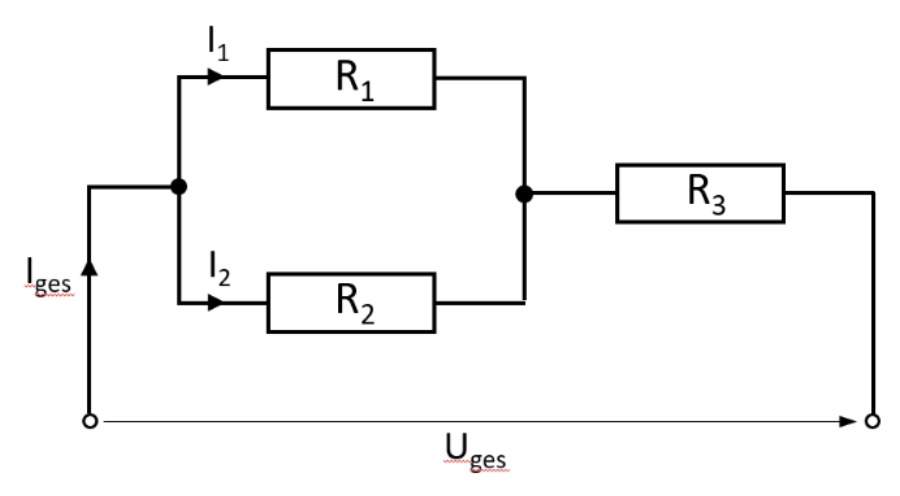
\includegraphics[width=0.5\textwidth]{bilder/Physik_04.png}
            \caption{Schaltkreis für Versuch 2}
            \label{fig:versuch2}
        \end{figure}

        Zunächst wird eine Spannung $U_{\mathrm{ges}} = 5\ \mathrm{V}$ an die Schaltung angelegt. Nun werden die Teilspannung $U_{3}$ und der Teilstrom $I_{2}$ gemessen und anhand dieser Messungen die restlichen Werte berechnet. Die Messwerte werden in Tabelle \ref{tab:versuch2} festgehalten.
        Danach wird der Versuch wiederholt, jedoch wird die Spannung so gewählt, das eine Stromstärke von $I_{mathrm{ges}} = 10\ \mathrm{mA}$ fließt. Die Messwerte werden ebenfalls in Tabelle \ref{tab:versuch2} festgehalten.

    \subsection{Ergebnisse}

        \begin{table}[h!]
            \centering
            \begin{tabular}{|l|l|l|l|l|l|l|l|l|l|l|}
                \hline
                $I_{\mathrm{ges}}$ in $\mathrm{mA}$ & $I_{1}$ in $\mathrm{mA}$ & $I_{2}$ in $\mathrm{mA}$ & $I_{3}$ in $\mathrm{mA}$ & $U_{\mathrm{ges}}$ in $\mathrm{V}$ & $U_{1}$ in $\mathrm{V}$ & $U_{2}$ in $\mathrm{V}$ & $U_{3}$ in $\mathrm{V}$ & $R_{1}$ in $\mathrm{\Omega}$ & $R_{2}$ in $\mathrm{\Omega}$ & $R_{3}$ in $\mathrm{\Omega}$\\
                \hline\hline
                $3,81$ & $2,41$ & $1,40$ & $3,81$ & $5,00$ & $0,60$ & $0,60$ & $3,80$ & $248,96$ & $428,57$ & $997,38$\\
                \hline
                $10,00$ & $6,10$ & $3,90$ & $10,00$ & $13,40$ & $1,63$ & $1,63$ & $10,14$ & $267,21$ & $417,95$ & $1014,00$\\
                \hline
            \end{tabular}
            \caption{Messwerte für Versuch 2}
            \label{tab:versuch2}
        \end{table}

        Die Berechnung der Werte erfolgt bei beiden Messungen nach folgdendem Schema. Zunächst lässt sich $I_{3}$ berechnen, da die Stromstäre in einer Reihenschaltung überall gleich ist und $I_{1}$, da sich die Stromstärke in Parallelschaltungen aufteilt und $I_{\mathrm{ges}}$ und $I_{2}$ gegeben sind.
        Danach lassen sich die Spannung $U_{1}$ und $U_{2}$ berechnen, da sich die beiden Widerstände als ganzes betrachtet in Reihe geschaltet sind und sich die Spannung auf jedes Element in einer Reihenschaltung aufteilt. Und in Parallelschaltungen ist die Spannung überall gleich.
        Zuletzt lassen sich die jeweiligen Widerstände mit der Formel berechnen:

        \begin{equation}
            R = \frac{U}{I}
        \end{equation}

        TODO: Diskussion

\section{Versuch 3: Wechselspannung und Oszilloskop}

    \subsection{Versuchsaufbau und -durchführung}
        
        In Versuch 3 wird mit einem Signalgenerator eine sinusförmige Wechselspannung mit $f = 40\ \mathrm{kHz}$ erzeugt. Diese soll mit dem Oszilloskop beobachtet werden. Anschließend soll eine Schirmskizze angefertigt werden und ausgewertet werden. Die Auswertung ist in Tabelle \ref{tab:versuch3} festgehalten. Als zweite Spannung wir eine rechteckförmige Wechselspannung mit $f = 2,5\ \mathrm{kHz}$ erzeugt. Die Auswertung ist ebenfalls in Tabelle \ref{tab:versuch3} festgehalten.
        Abbildungen \ref{fig:versuch3_1} und \ref{fig:versuch3_2} zeigen die Schirmskizzen.

    \subsection{Ergebnisse}

        TODO: Schirmskizzen

        \begin{table}[h!]
            \centering
            \begin{tabular}{|l|l|l|l|}
                \hline
                $f_{\mathrm{geg}}$ in $\mathrm{kHz}$ & Amplitude in $\mathrm{V}$ & Periode $T$ in $\mathrm{\mu s}$ & Frequenz $f$ in $\mathrm{kHz}$\\
                \hline\hline
                $40,0$ & $6,2 \pm 0,4$ & $25,0 \pm 1,0$ & $40,0 \pm 1,6$\\
                \hline
                $2,5$ & $2,0 \pm 0,2$ & $400,0 \pm 20,0$ & $2,5 \pm 0,125$\\
                \hline
            \end{tabular}
            \caption{Auswertung für Versuch 3}
            \label{tab:versuch3}
        \end{table}

        Die Fehlerberechnung ergibt sich aus dem Größtfehler:

        \begin{equation}
            \Delta f = \frac{1}{T^2} \cdot \Delta \mathcal{T}
        \end{equation}

        mit $\Delta \mathcal{T} = 1\ \mathrm{\mu s}$, bzw. $\Delta \mathcal{T} = 20\ \mathrm{\mu s}$. Die Amplitude besitzt einen Fehler von $0,4\ \mathrm{V}$, bzw. $0,2\ \mathrm{V}$. Der Fehler der Amplitude ist allerdings nicht für die Berechnung der Frequenz relevant.

        TOD: Diskussion

\section{Versuch 4: Ladeverhalten eines Kondensators}

    \subsection{Versuchsaufbau und -durchführung}

        TODO: Versuchsaufbau und -durchführung
        Ohmscher Widerstand $R = 100\ \mathrm{\Omega}$

    \subsection{Ergebnisse}
        
        \begin{table}[h!]
            \centering
            \begin{tabular}{|l|l|l|l|}
                \hline
                $n$ & Zeit $t$ in $\mathrm{ms}$ & Amplitude in $V$ & $I$ in $A$\\
                \hline\hline
                $1$ & $0,000$ & $6,48$ & $0,0648$\\
                \hline
            \end{tabular}
            \caption{Messwerte für Versuch 4}
            \label{tab:versuch4}
        \end{table}

        \begin{figure}[h!]
            \centering
            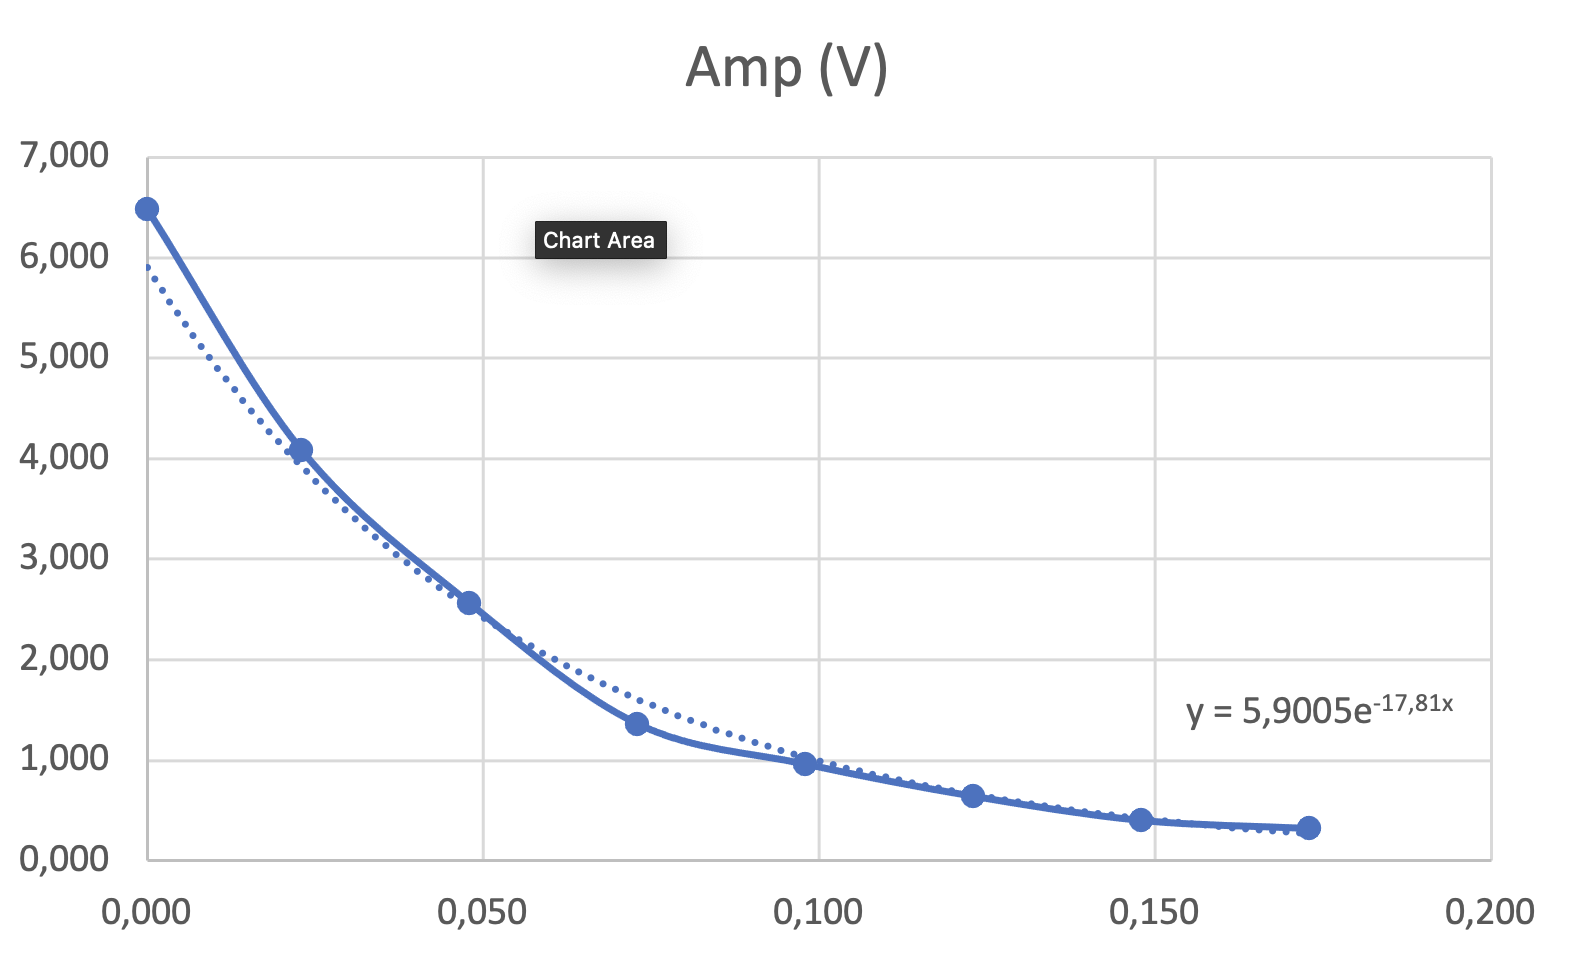
\includegraphics[width=0.5\textwidth]{bilder/Physik_05.png}
            \caption{Schirmskizze für Versuch 4}
            \label{fig:versuch4}
        \end{figure}

        TODO: Berechnung von $C$
        TODO: Diskussion